\subsection{Cross-validated results}
The CNN models were trained using an ADAM-optimizer, a batch size of $30$ and the Area Under the Curve (AUC)-score, on the validation set, was used to reduce the learning rate during training. The learning rate was initially at $0.001$ for all models and decreased by a factor of 10, each epoch that the AUC score did not improve. Early stopping was used to stop training when the AUC score, on the validation data, did not improve over two successive epochs.

The ensemble models were trained using n\_estimators $=$ 5 for the random forest classifier and the input features were scaled using a Standard Scaler \cite{pedregosa_scikit-learn_2011}.

All models were scored using F1, F2, G2 and PhysioNet CinC Challenge score for each of the 10-folds \footnote{All codes and models are available here: \url{https://github.com/Bsingstad/FYS-STK4155-oblig3}}. The results in figure \ref{fig:crossval_score} show that the random forest-based ensemble model, using features from all 12 leads, outperformed the other models on all metrics used in this study. 



\newpage
\begin{figure}[ht!]
\vspace{0em}
  \subfloat[(a) F1-score]{
	\begin{minipage}[c][1\width]{
	   0.5\textwidth}
	   \centering
	   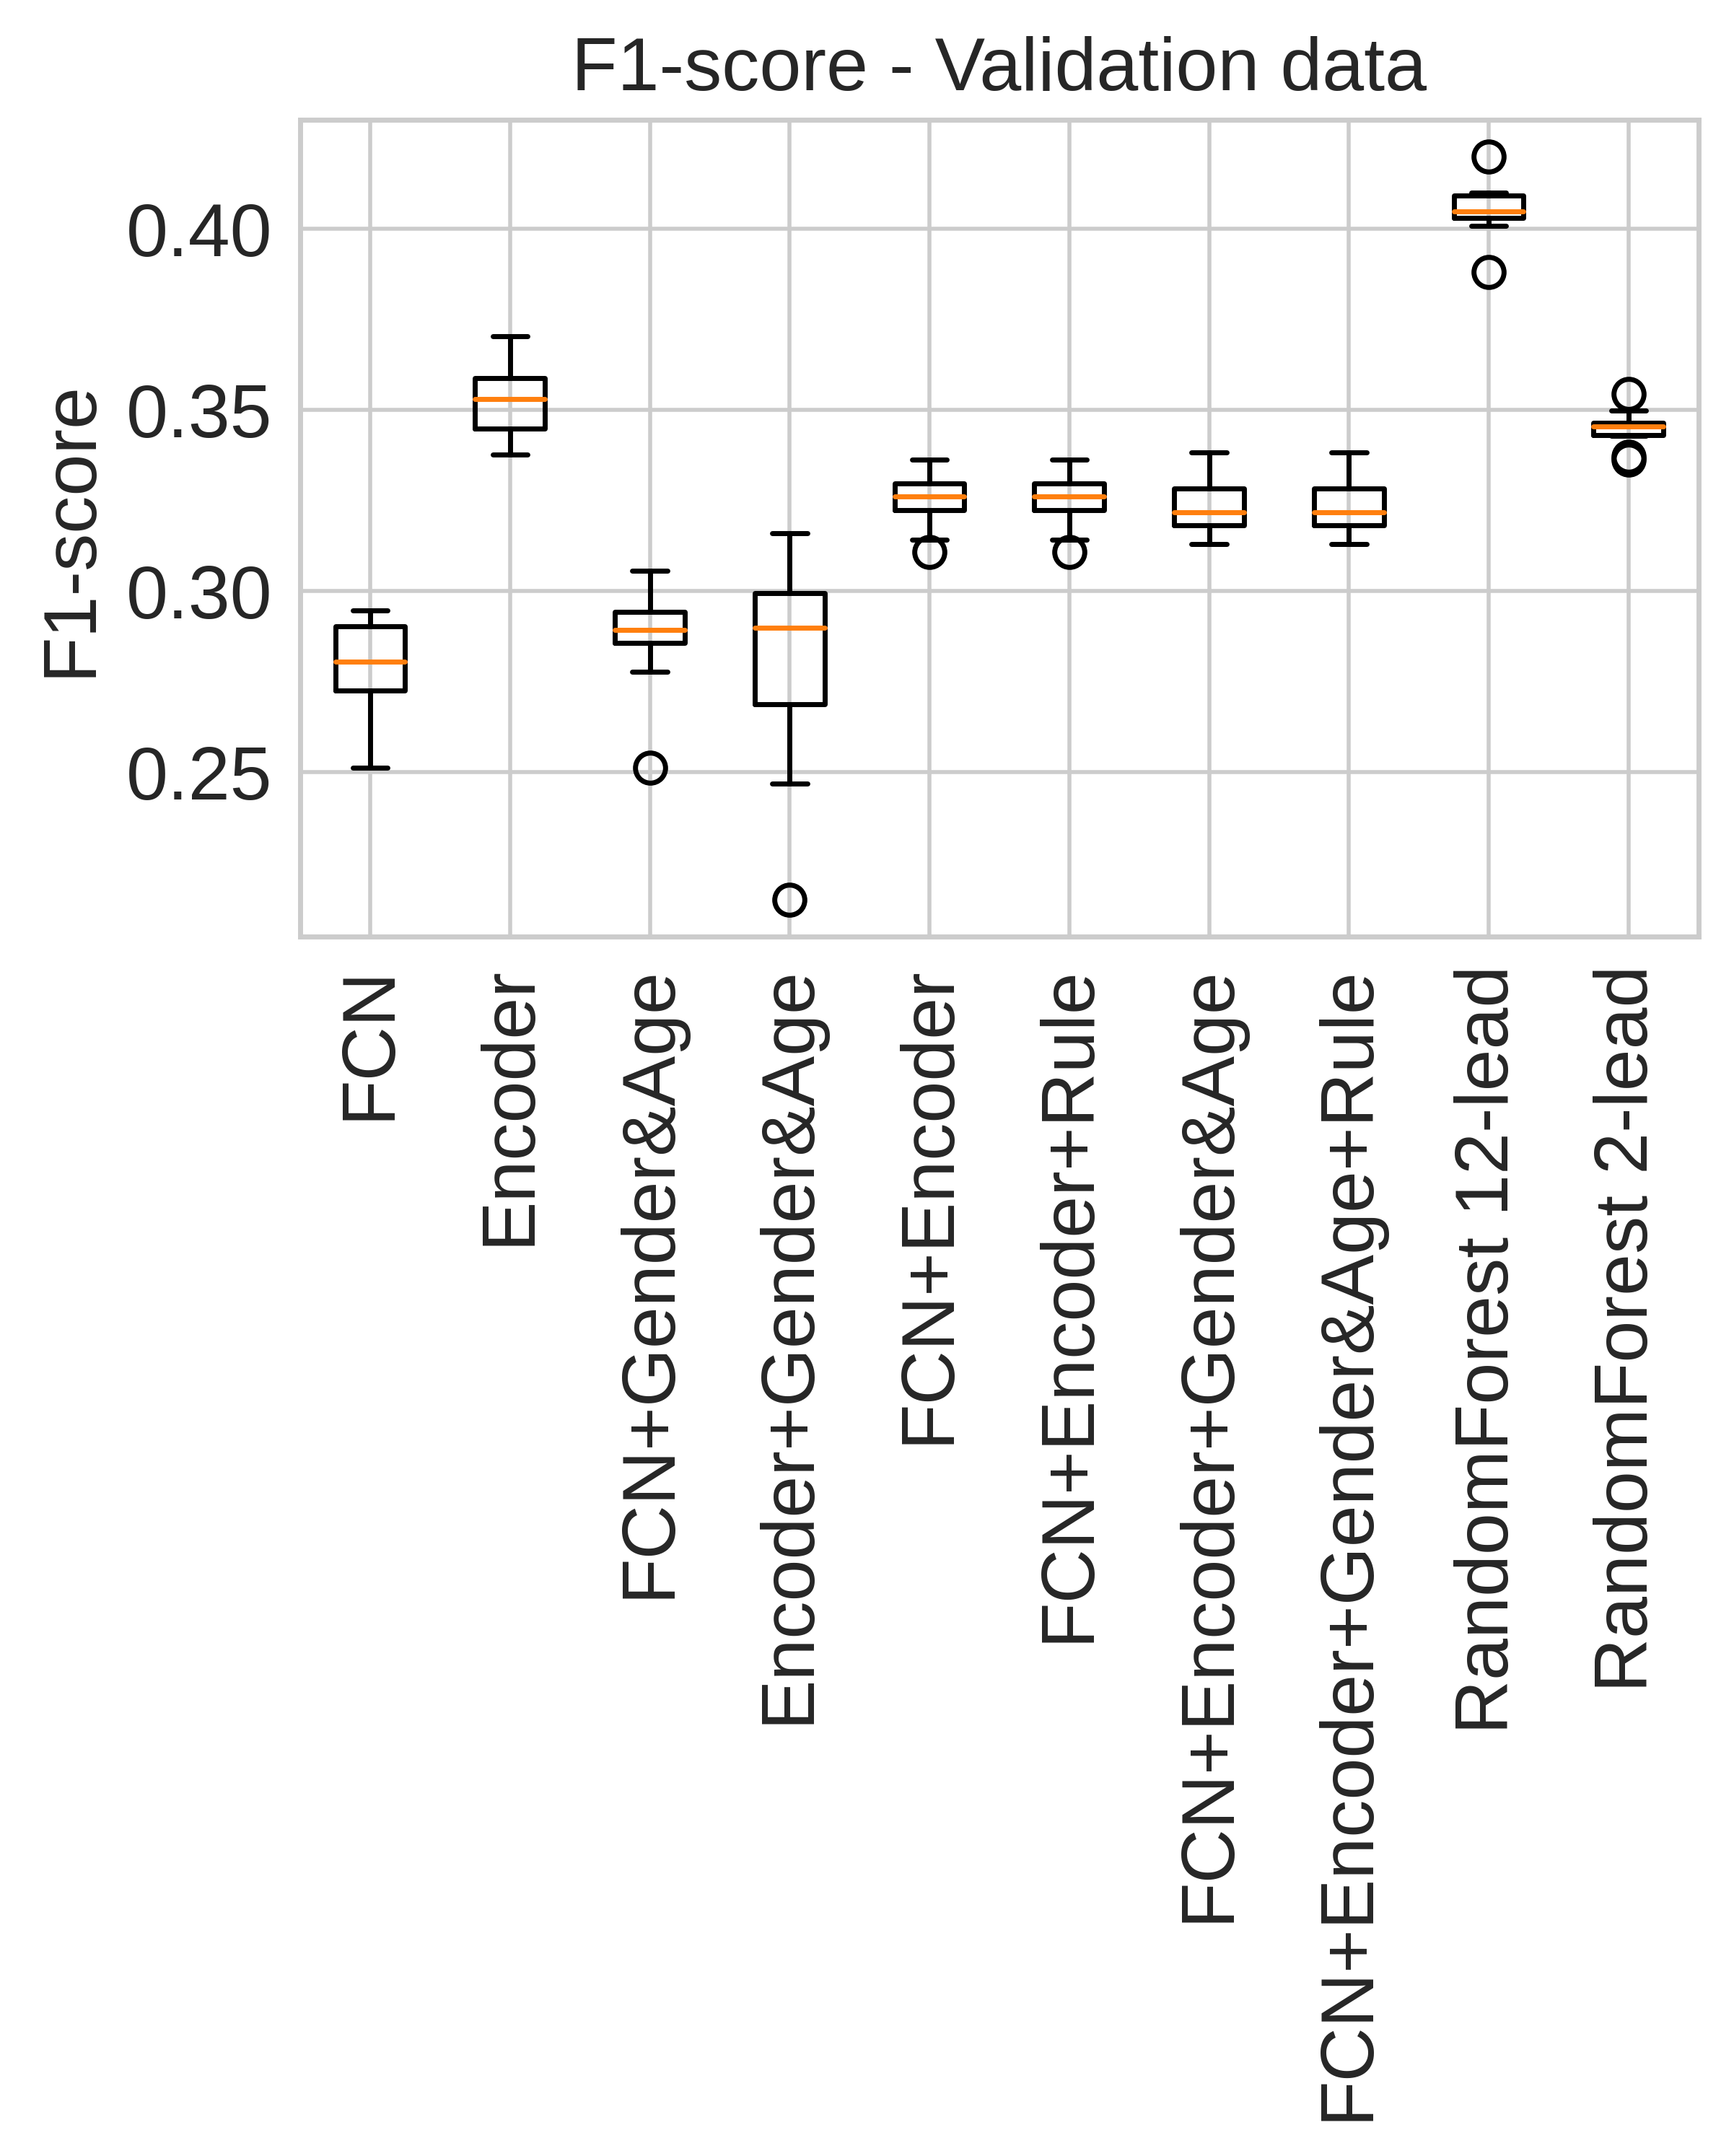
\includegraphics[width=0.9\textwidth]{Figures/F_score_val}
	   \vspace{0em}
	\end{minipage}}
 \hfill 	
  \subfloat[(b) F2-score]{
	\begin{minipage}[c][1\width]{
	   0.5\textwidth}
	   \centering
	   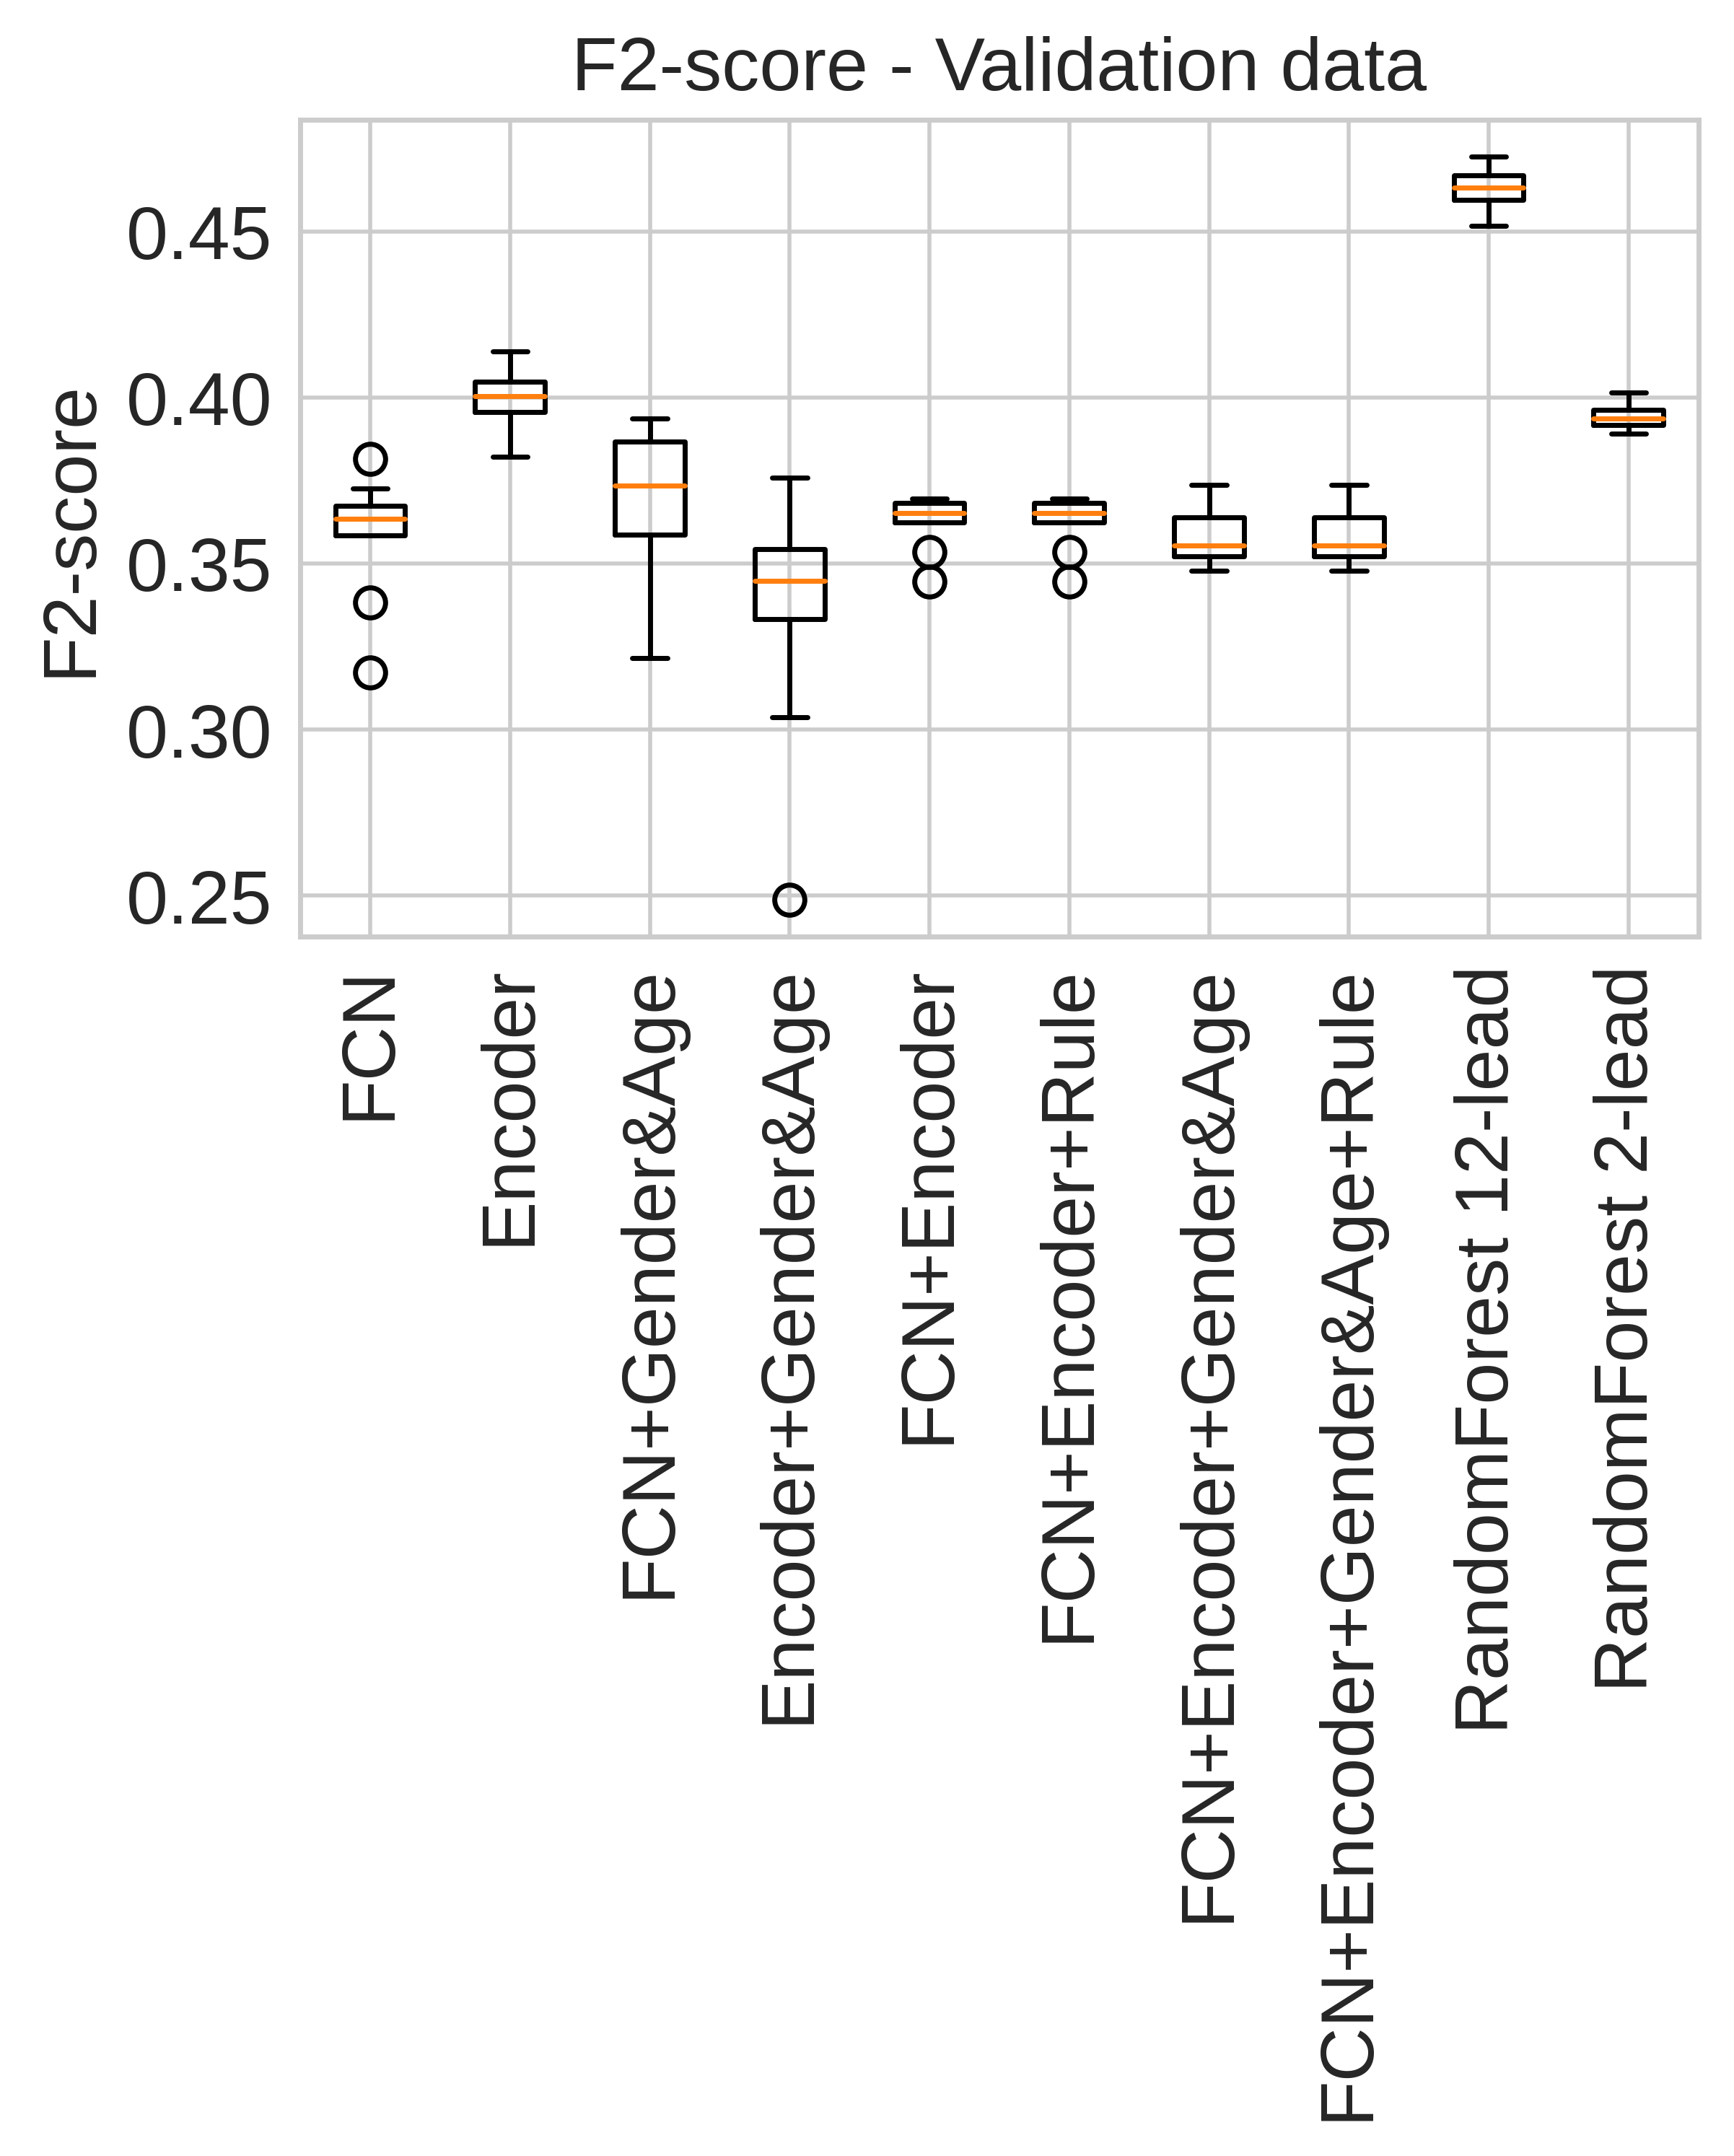
\includegraphics[width=0.9\textwidth]{Figures/F2_score_val}
	   \vspace{0em}
	\end{minipage}}
\end{figure}

\begin{figure}[hb!]
\vspace{0em}
  \subfloat[(c) G2-score]{
	\begin{minipage}[c][1\width]{
	   0.5\textwidth}
	   \centering
	   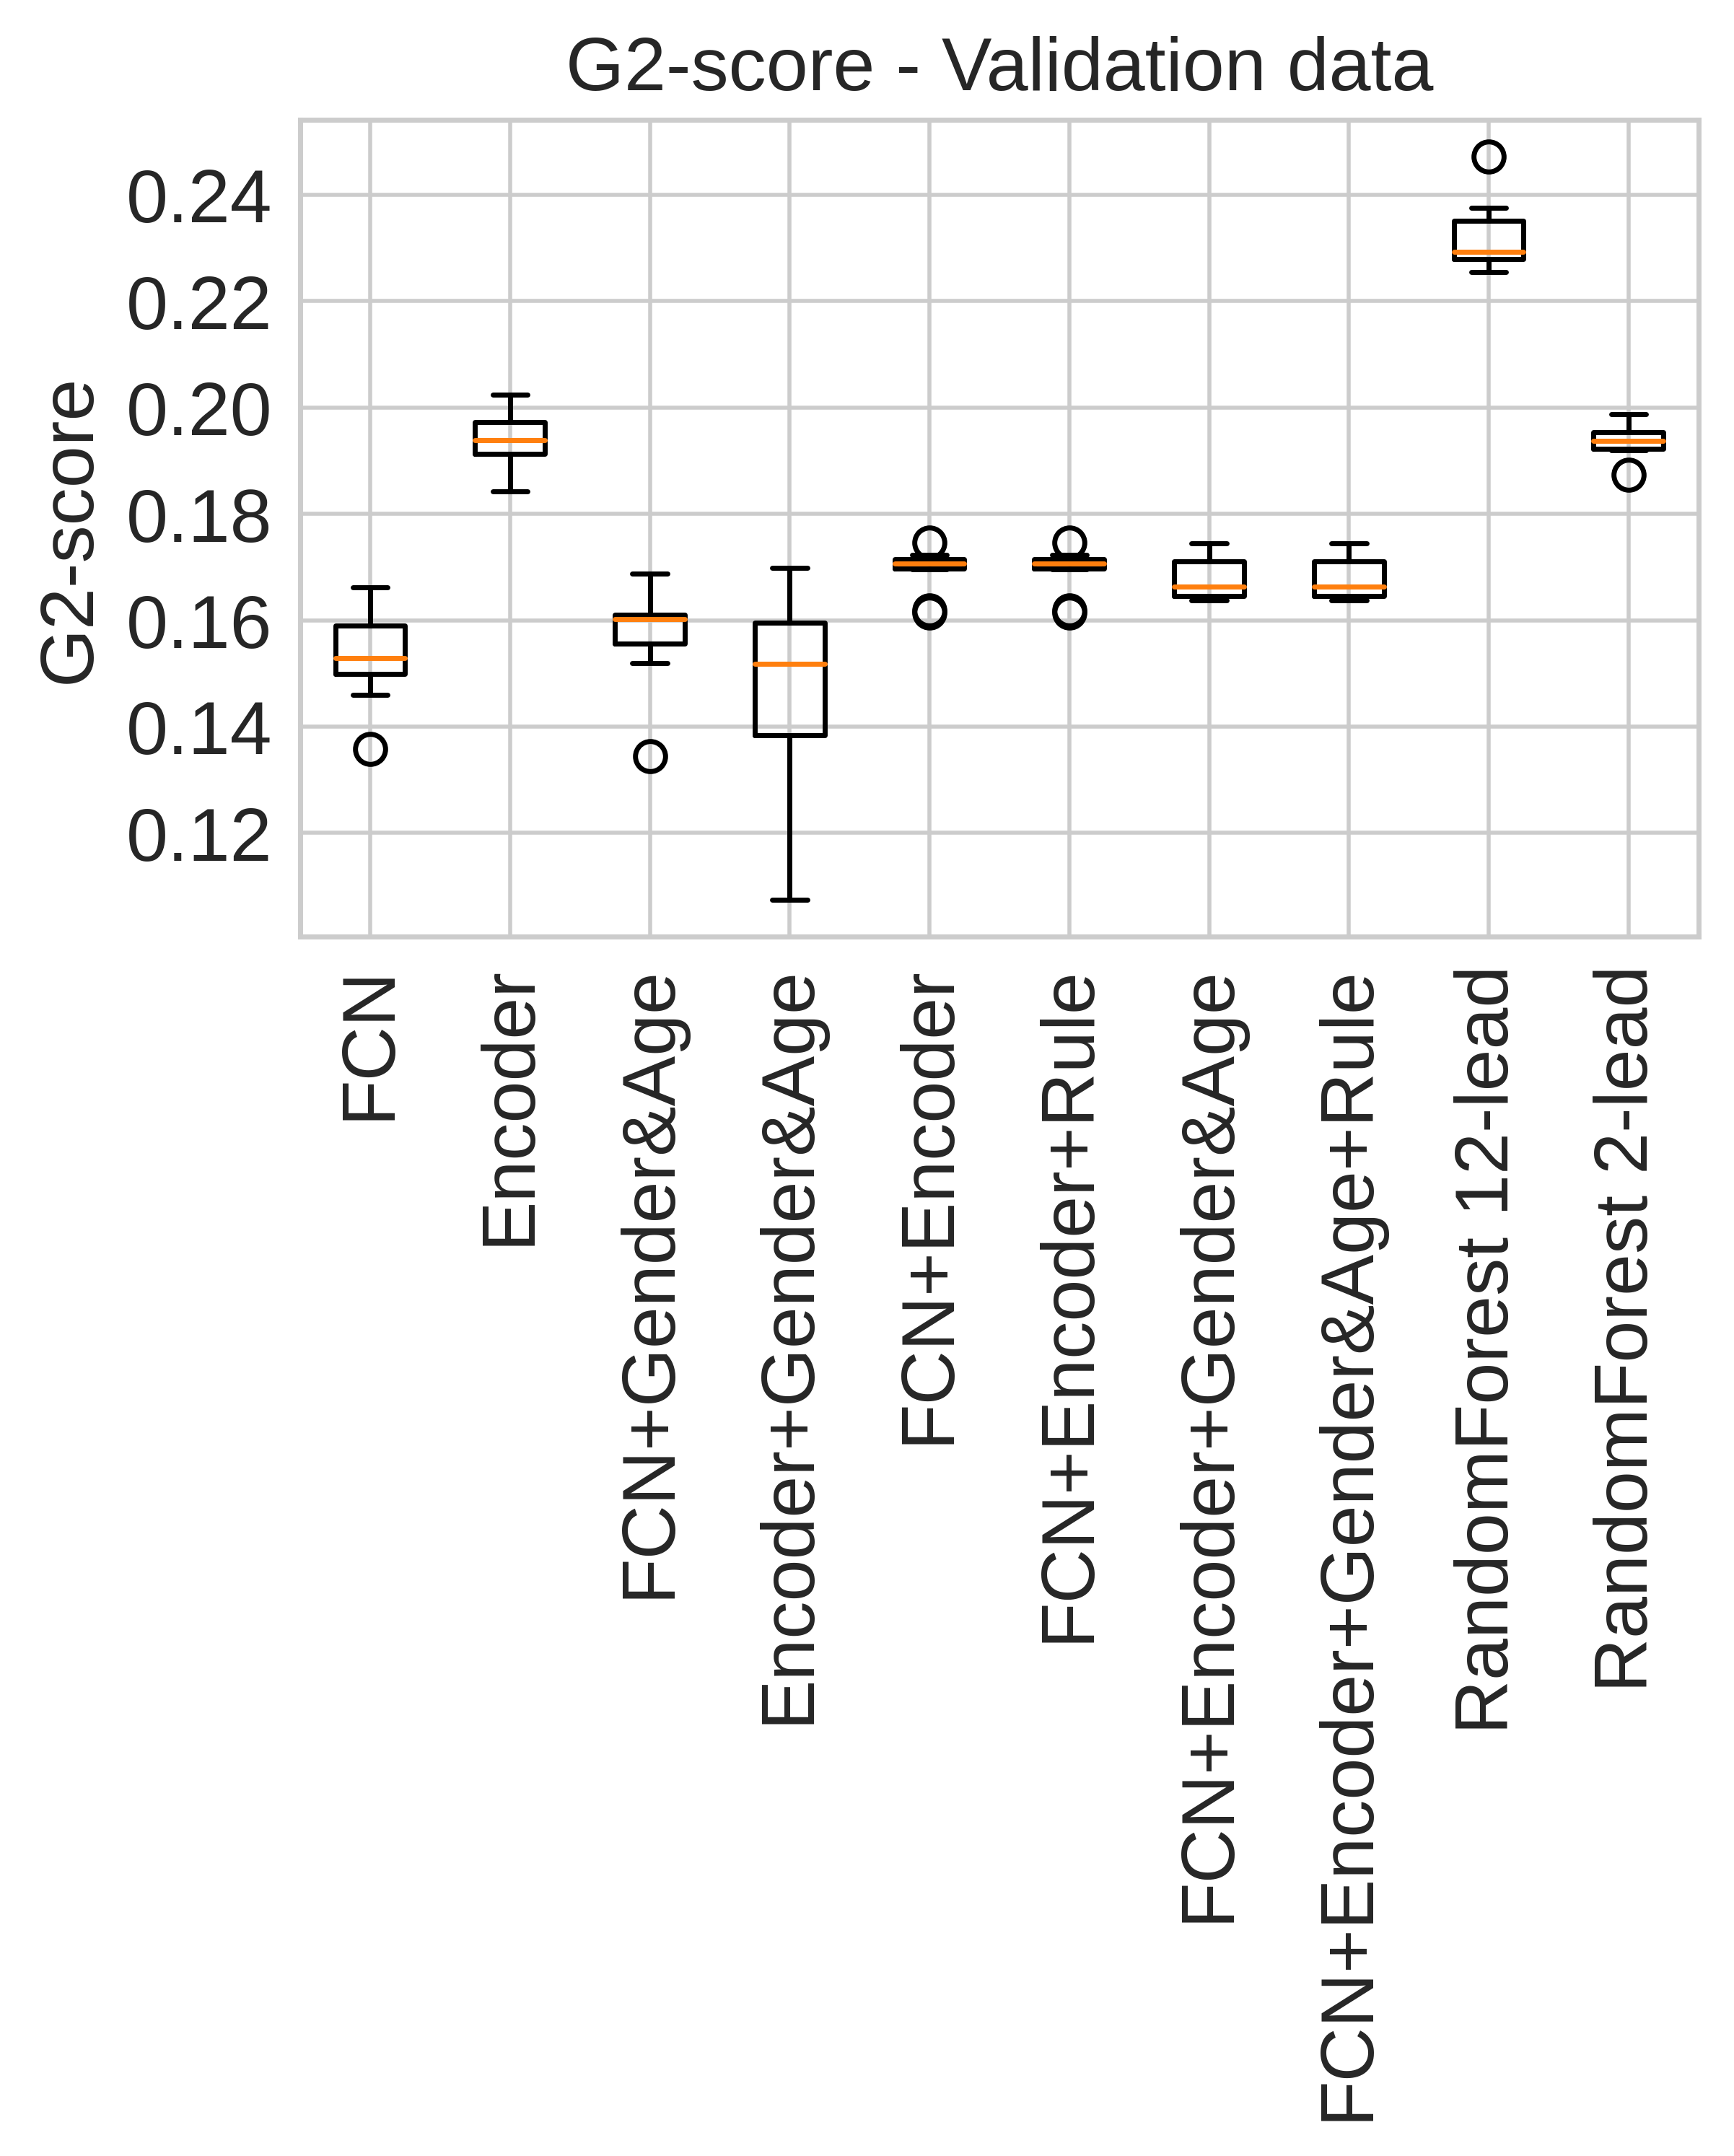
\includegraphics[width=0.9\textwidth]{Figures/G2_score_val}
	   \vspace{1em}
	\end{minipage}}
 \hfill 	
  \subfloat[(d) PhysioNet/CinC Challenge-score]{
	\begin{minipage}[c][1\width]{
	   0.5\textwidth}
	   \centering
	   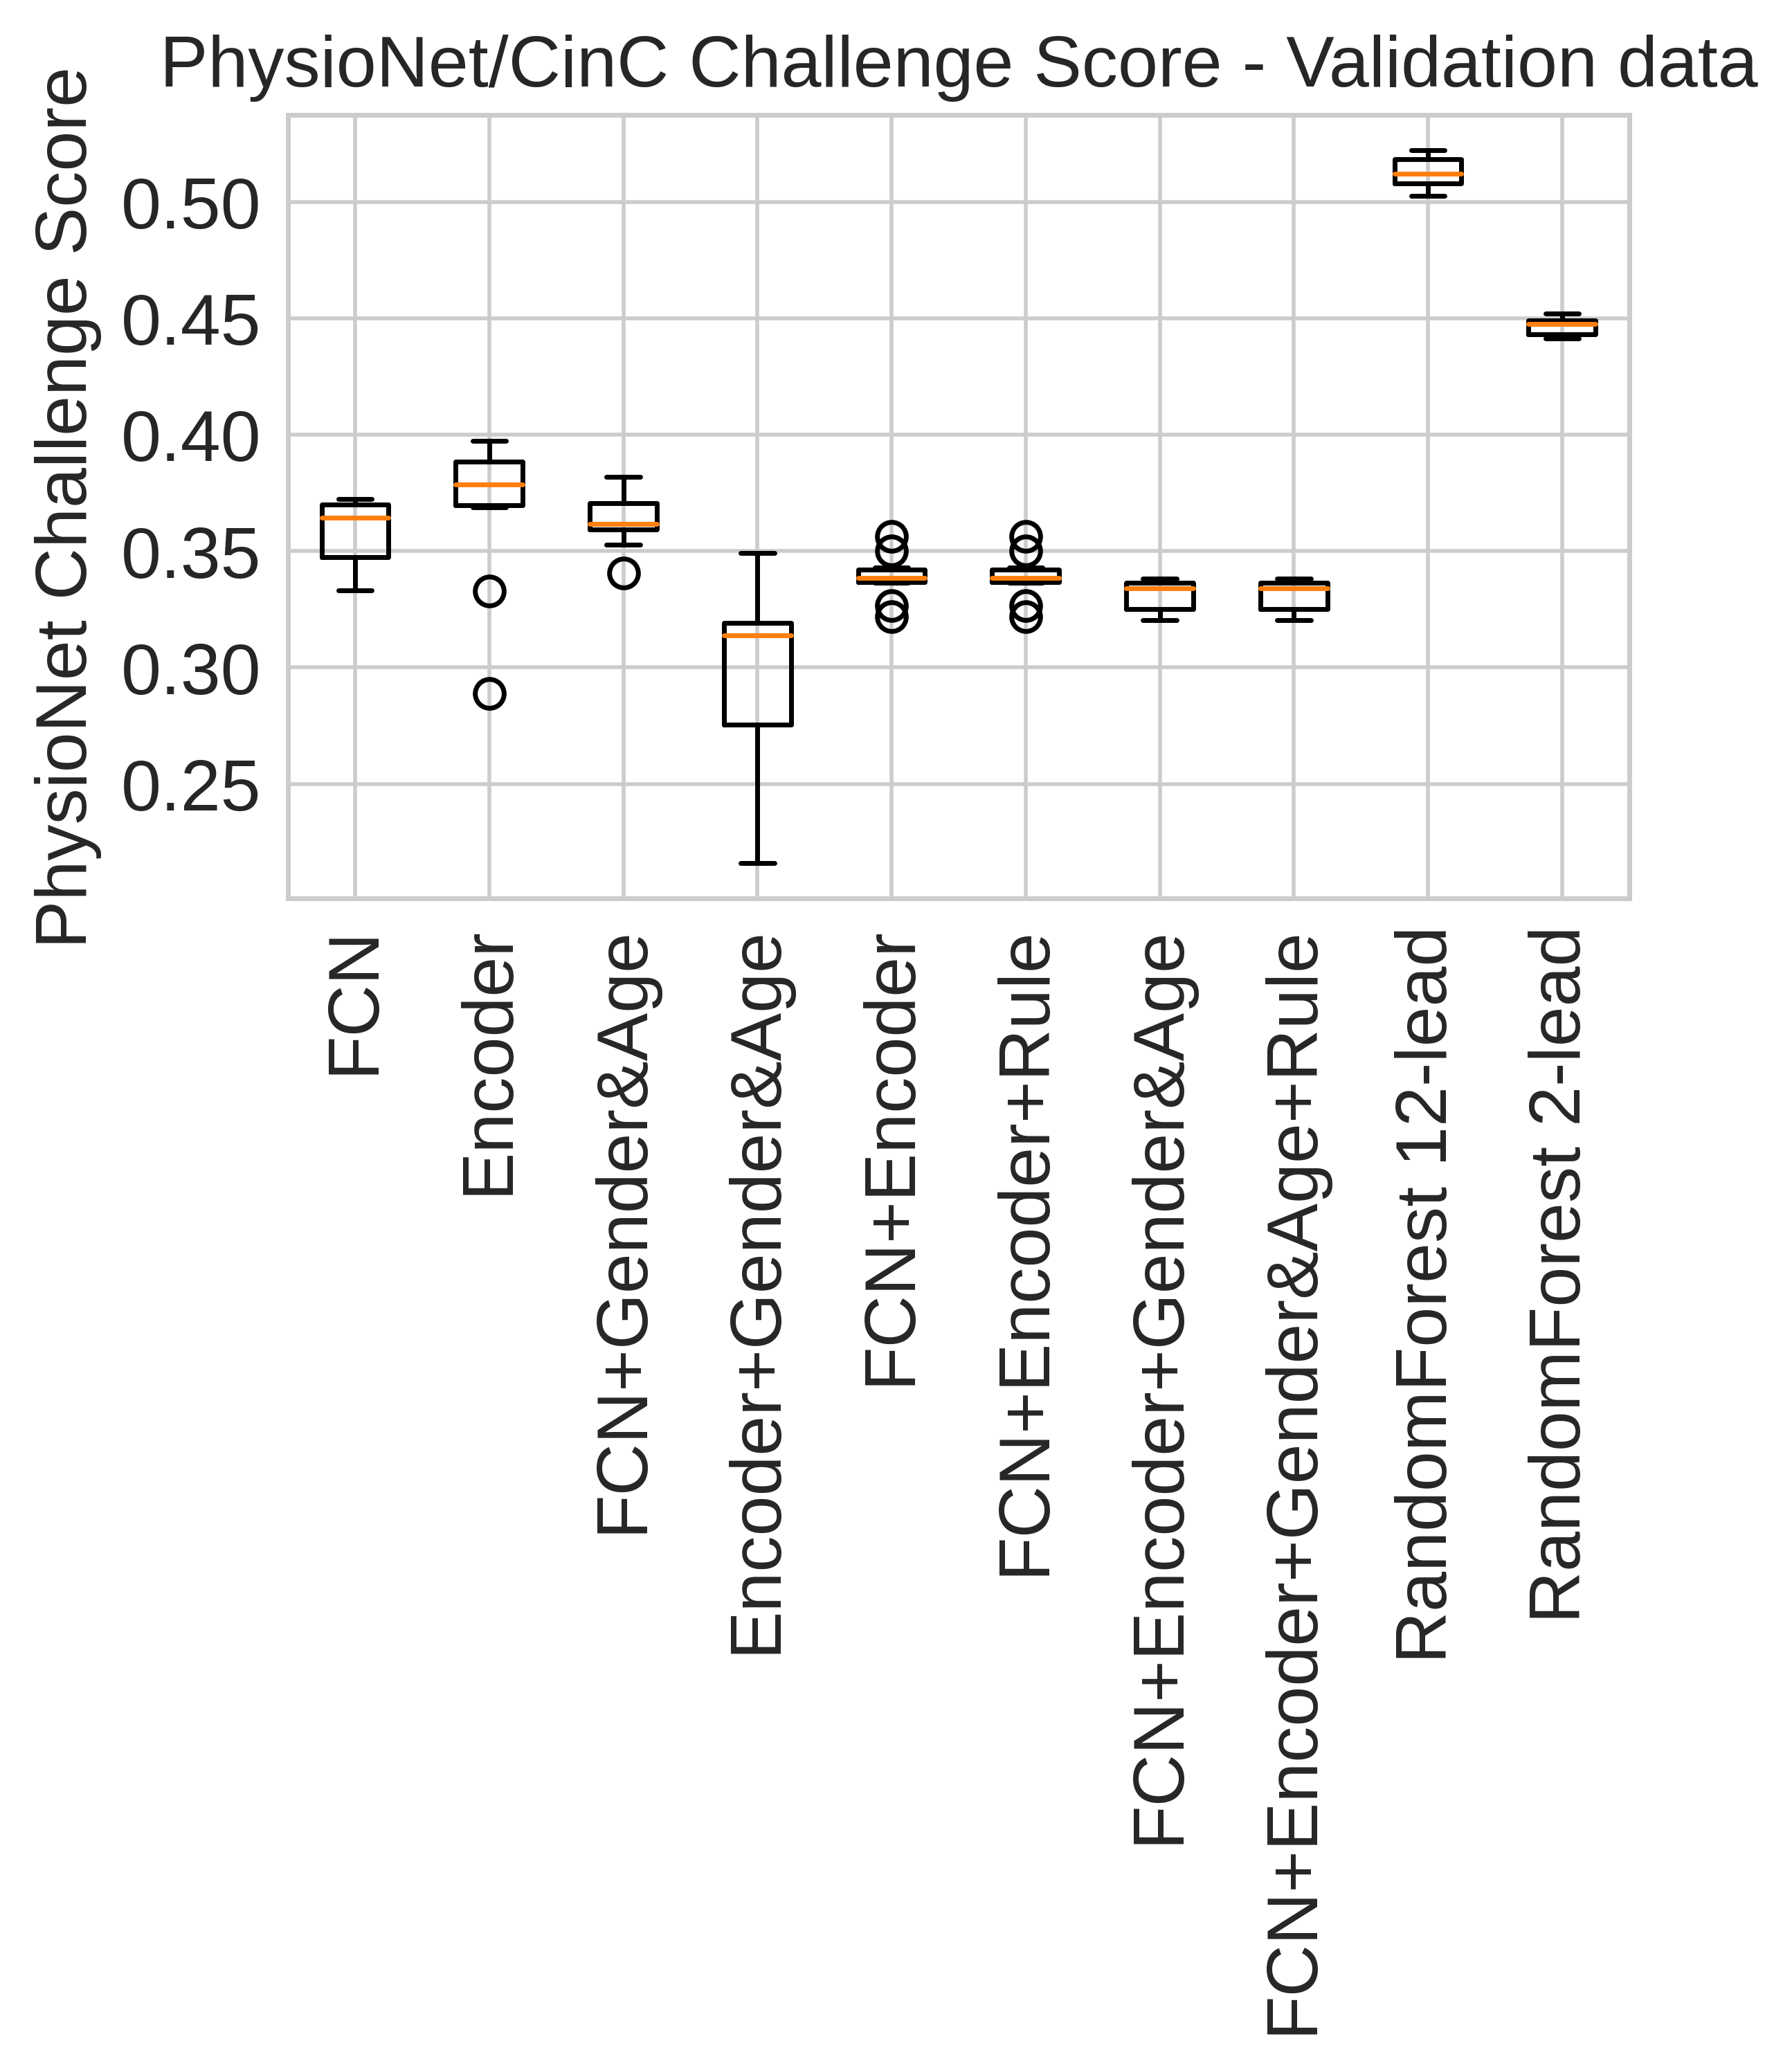
\includegraphics[width=0.9\textwidth]{Figures/PhysioNetChallenge_score_val}
	   \vspace{0em}
	\end{minipage}}
    \caption{The figure shows 10-fold cross-validated scores achieved by ten different models. The upper left shows F1-score, the upper right show F2-score, the lower-left shows G2-score and the lower right shows PhysioNet/CinC Challenge score. The PhysioNet/CinC Challenge score is described in \cite{alday_classification_2020}. The models referred to as ensemble models in this study are named \textit{RandomForest 12-lead} and \textit{RandomForest 2-lead} in this figure.}
\label{fig:crossval_score}
\end{figure}



\subsection{Explainability results}
The tabular explainer that was applied to the ensemble model was trained on $5000$ ECGs from the training data and then tested on an ECG from the test data. The ECG that was explained by the LIME tabular explainer was from a patient with atrial fibrillation. The explanation is visualized in figure \ref{fig:explainability_rand_12}.

%\begin{figure}[!bp]
%    \centering
%    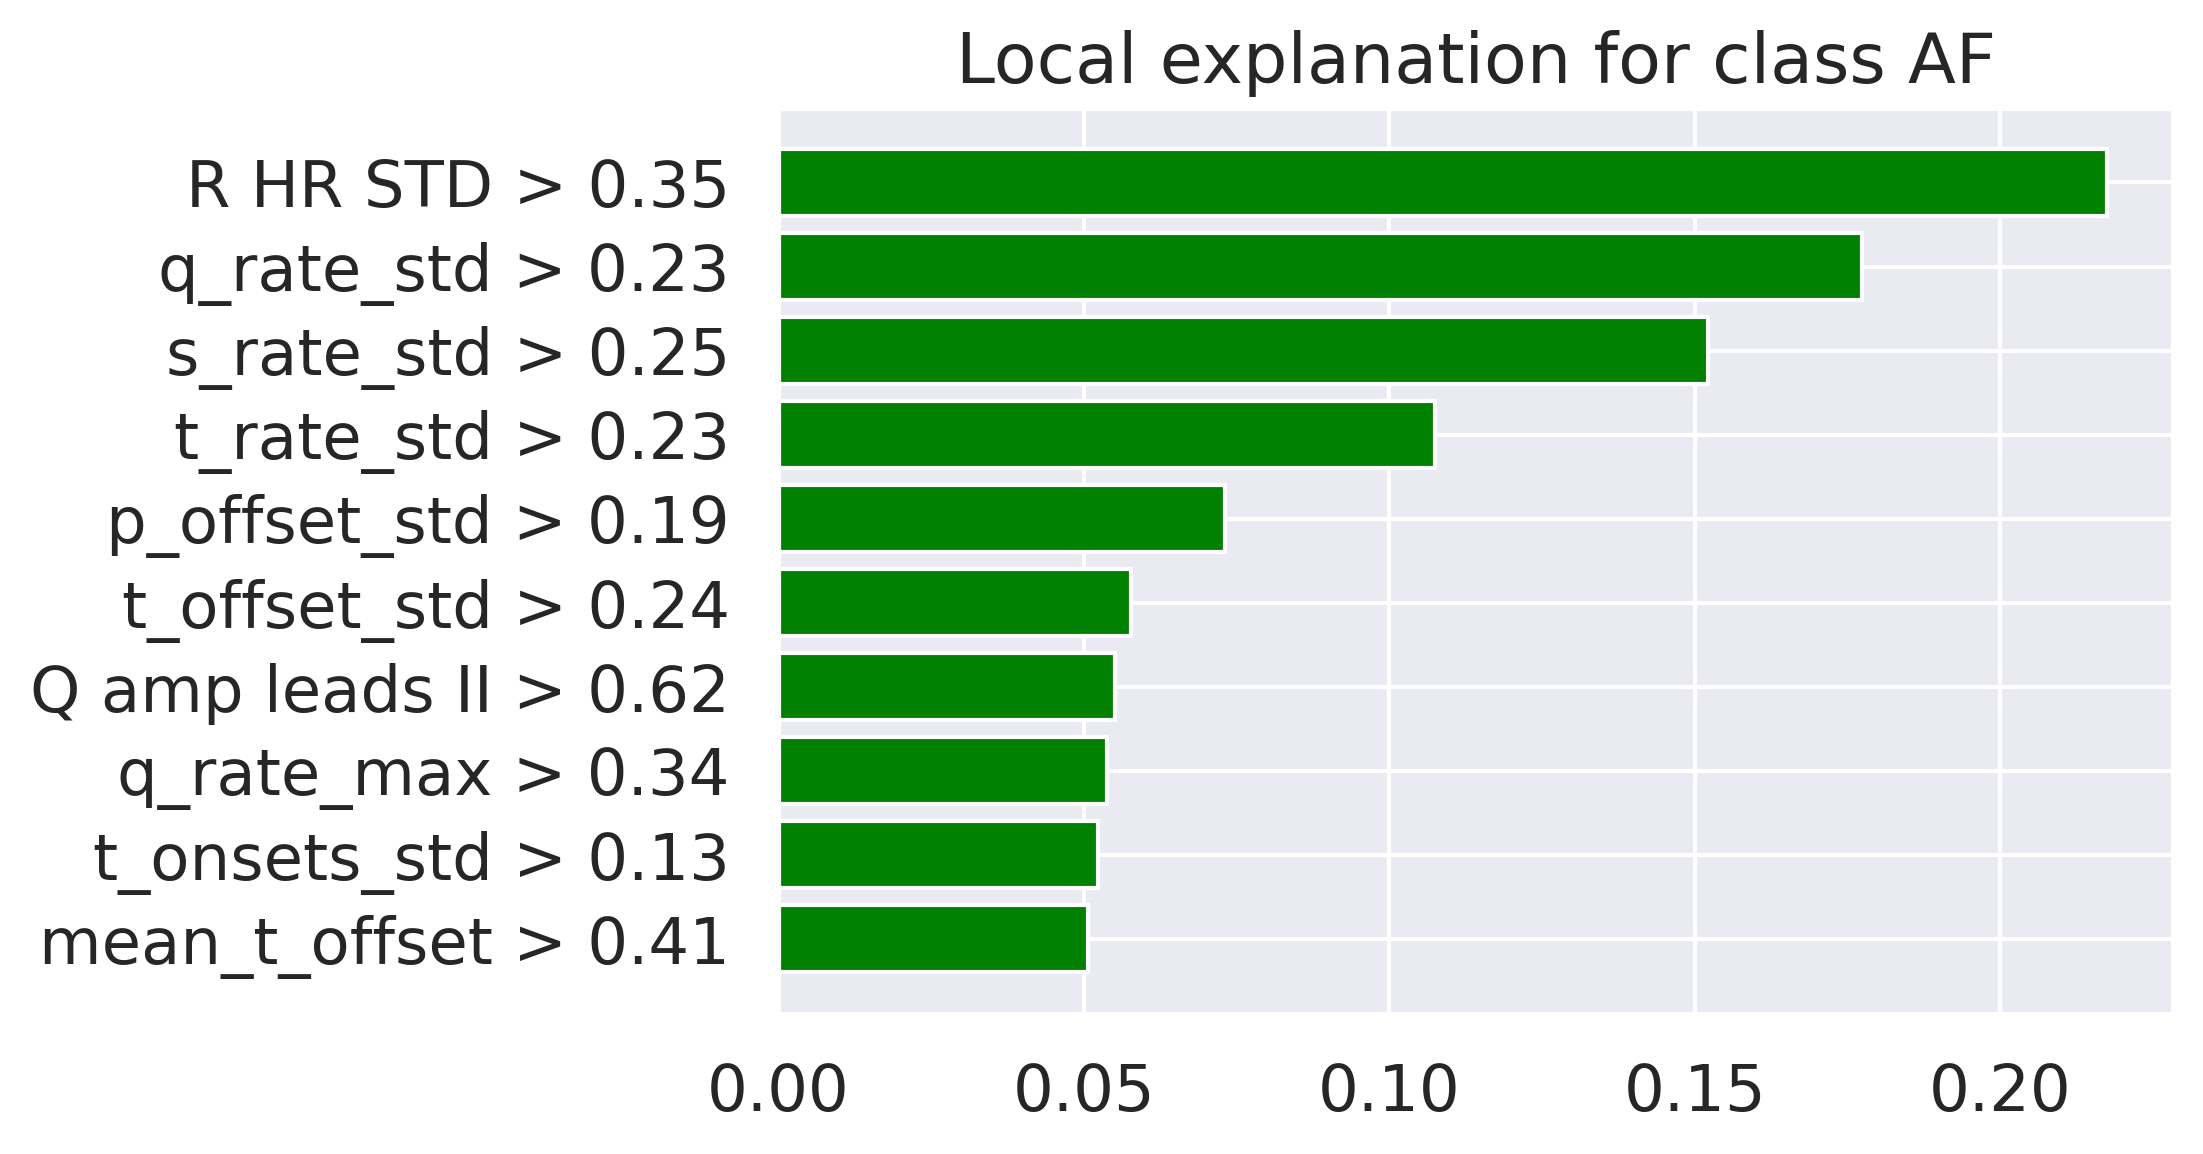
\includegraphics[width=0.8\textwidth]{Figures/atrialfib_atrialfib.png}
%    \caption{}
%    \label{fig:parameterregel}
%\end{figure}



\begin{figure}[!htp]
    \centering
    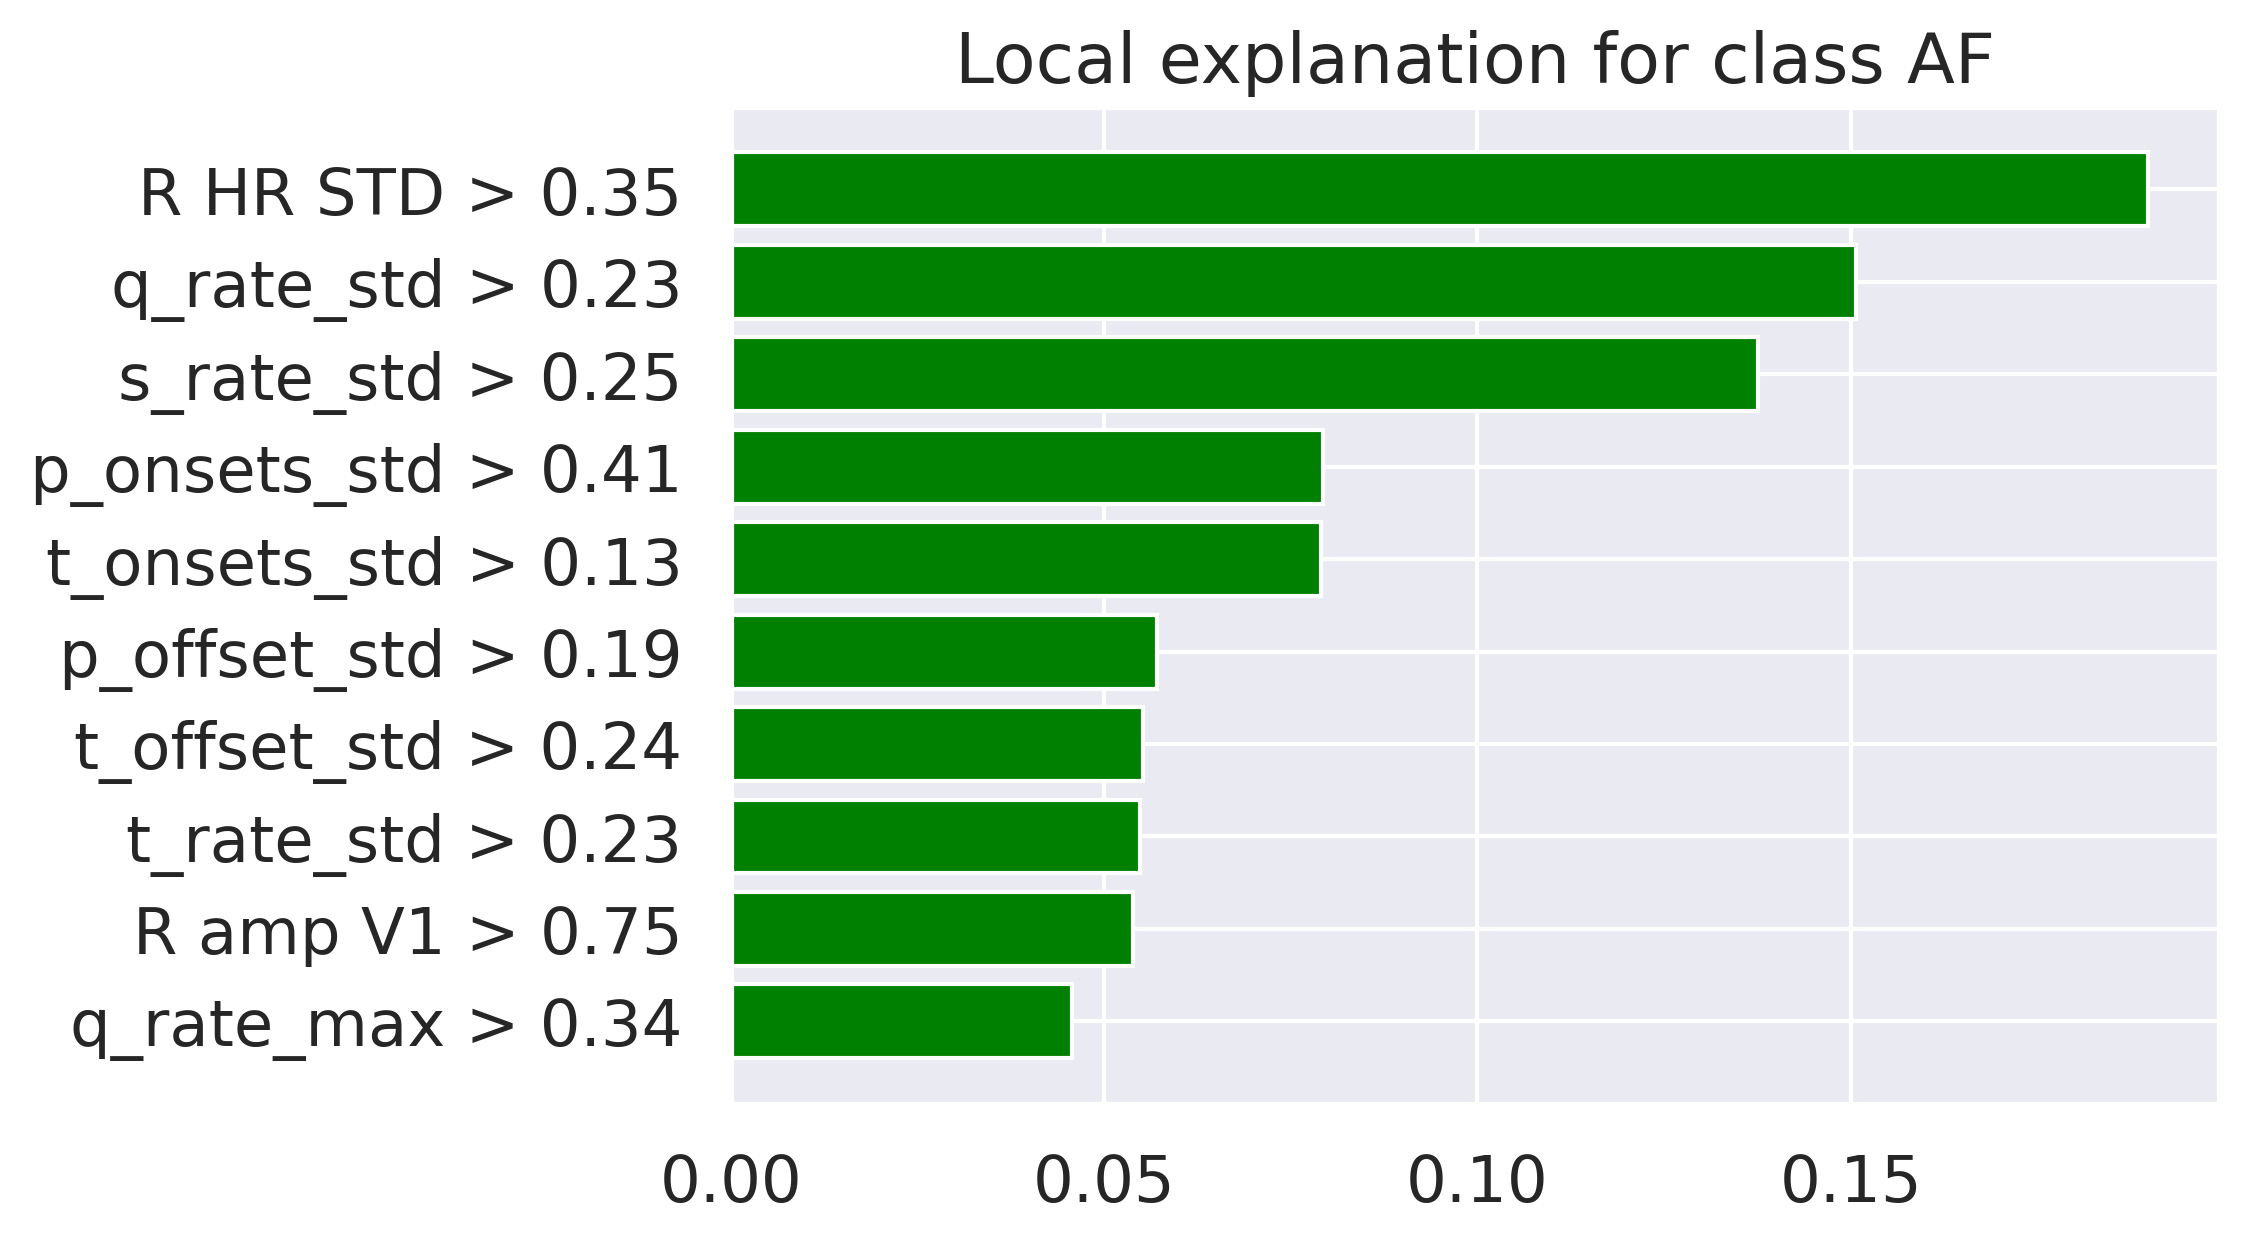
\includegraphics[width=.90\textwidth]{Figures/Atrialfib.png}
    \caption{The figure shows the top $10$ features from an ECG diagnosed with atrial fibrillation (AF). The ECG was correctly classified by the ensemble model. The green bars indicate the degree of contribution towards a positive classification of AF, while the red bars would have been shown if some features contributed towards a negative prediction of AF.
    In the labels on the vertical axis; amp is short for amplitude, std is short for standard deviation, HR is short for heart rate, P, Q, R,S,T are the characteristic peaks in the ECG and $I$, $II$, $III$, aVL, aVF, aVR, V1, V2, V3, V4, V5 and V& are the name of the 12 ECG leads.}
    \label{fig:explainability_rand_12}
\end{figure}








%\begin{figure}[!htp]
%   \centering
%    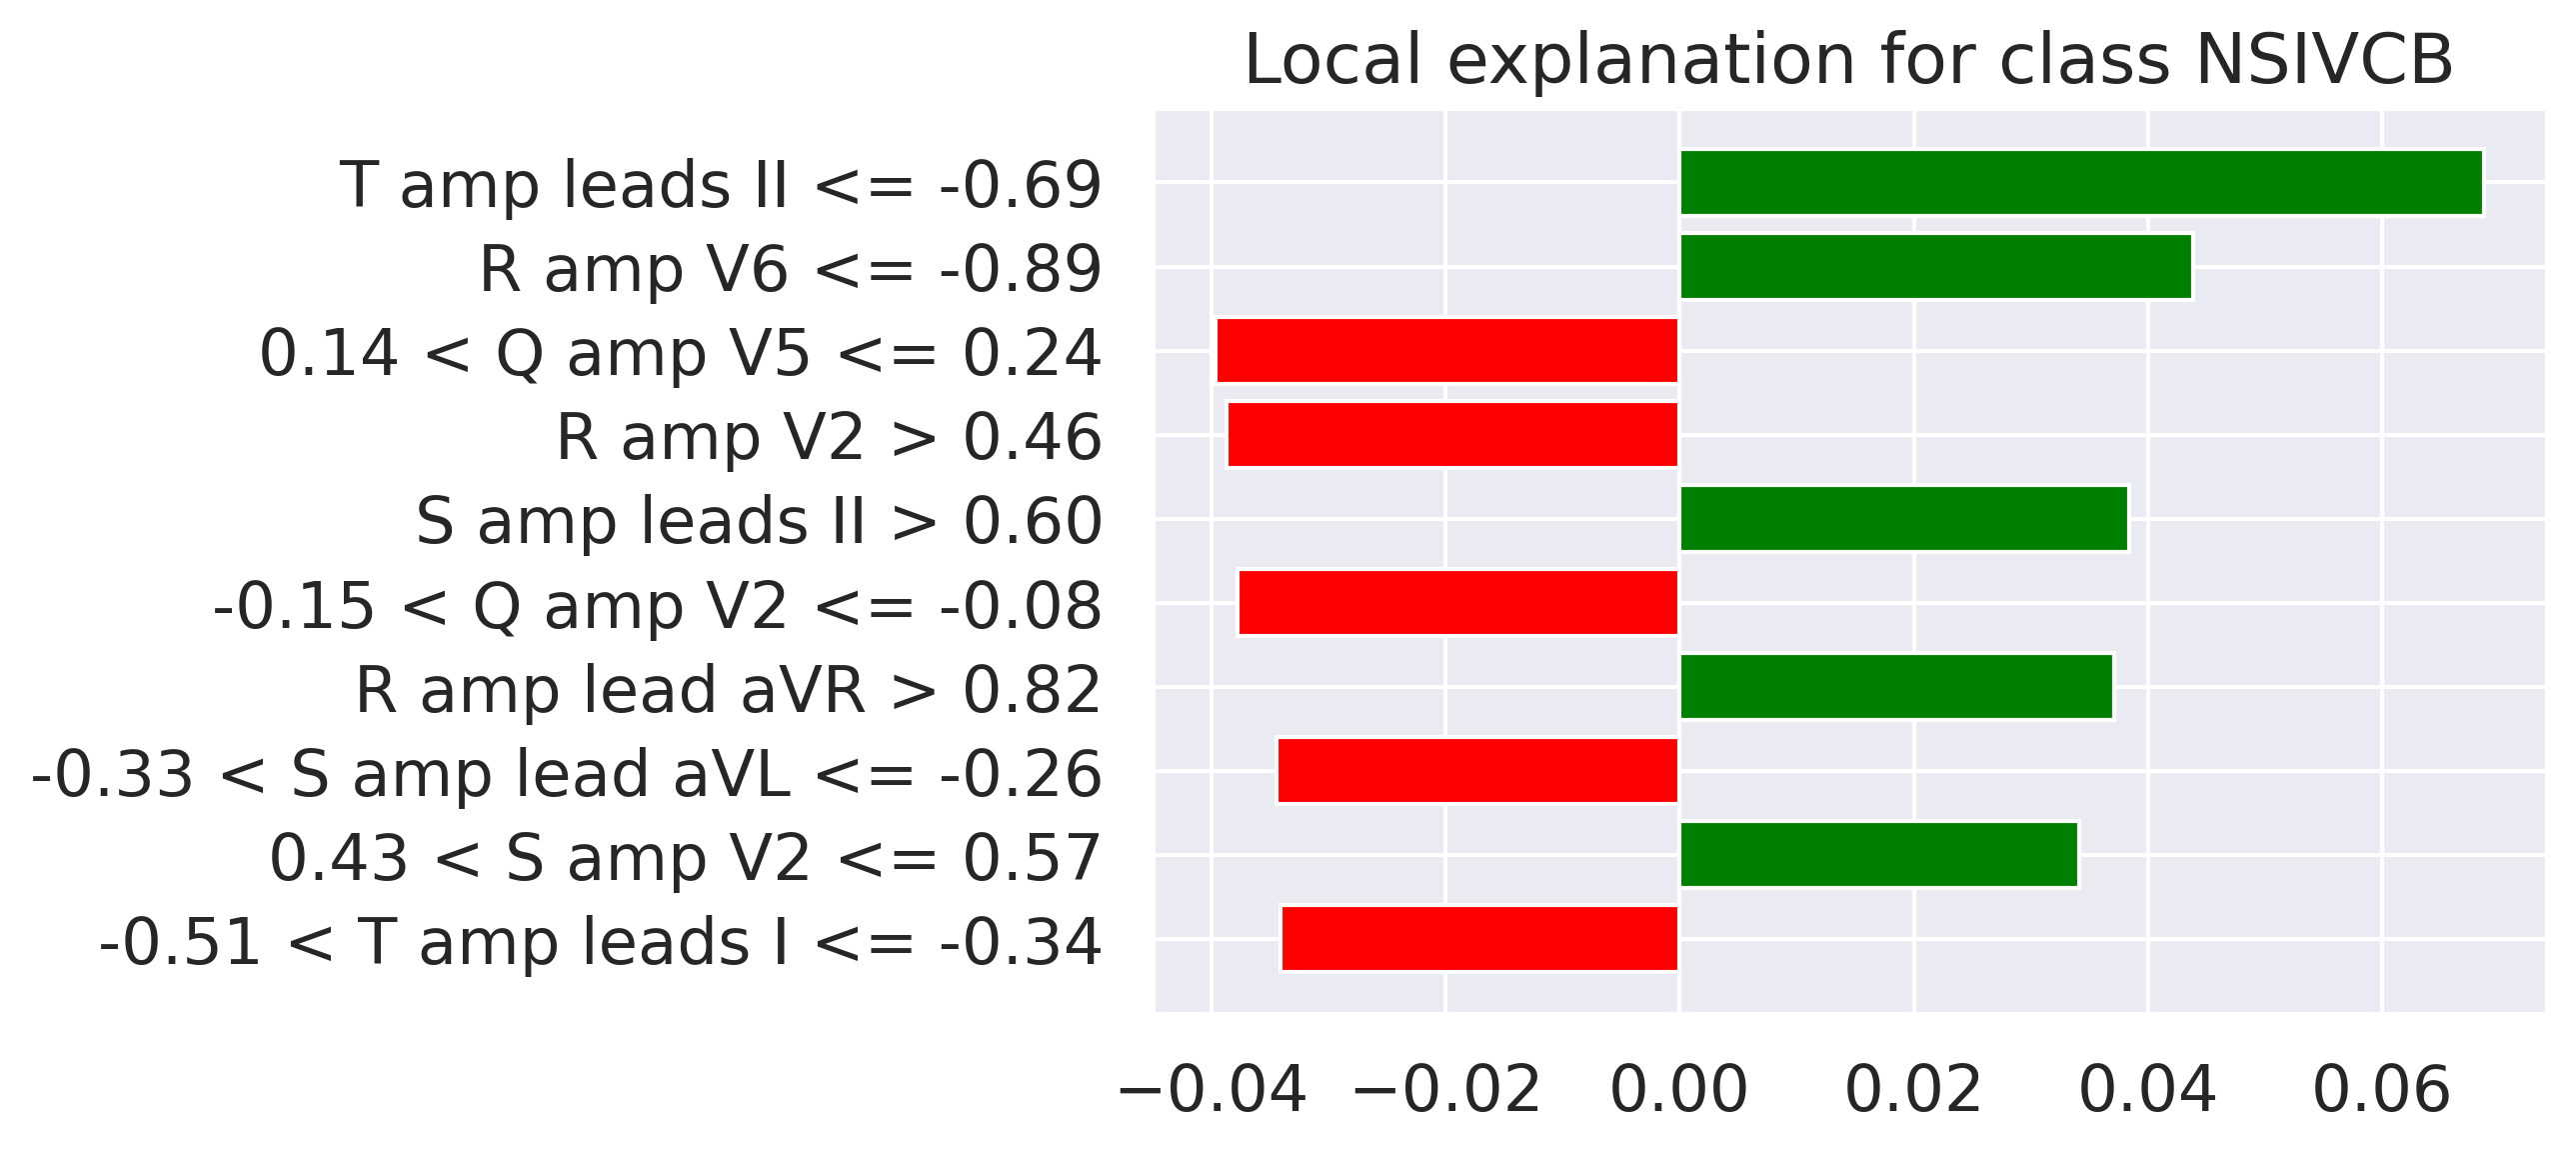
\includegraphics[width=.90\textwidth]{Figures/conduction_disorder_12lead.png}
%    \caption{The figure shows the top $10$ features from a ECG that contributed with the prediction. In the labels on the vertical axis; amp is short for amplitude, P, Q, R,S,T are the characteristic peaks in the ECG and $I$, $II$, $III$, aVL, aVF, aVR, V1, V2, V3, V4, V5 and V& are the name of the 12 ECG leads. The ECG-features are extracted from a ECG from a patient with non-specific intra ventricular conduction disorder (NSIVCB).  The green bars indicate the the degree of contribution towards an positive classification of NSIVCB, while the red bars shows the degree of contribution towards a negative classification of NSIVCB.}
%    \label{fig:explainability_rand_12}
%\end{figure}
%\begin{figure}[!bp]
%    \centering
%    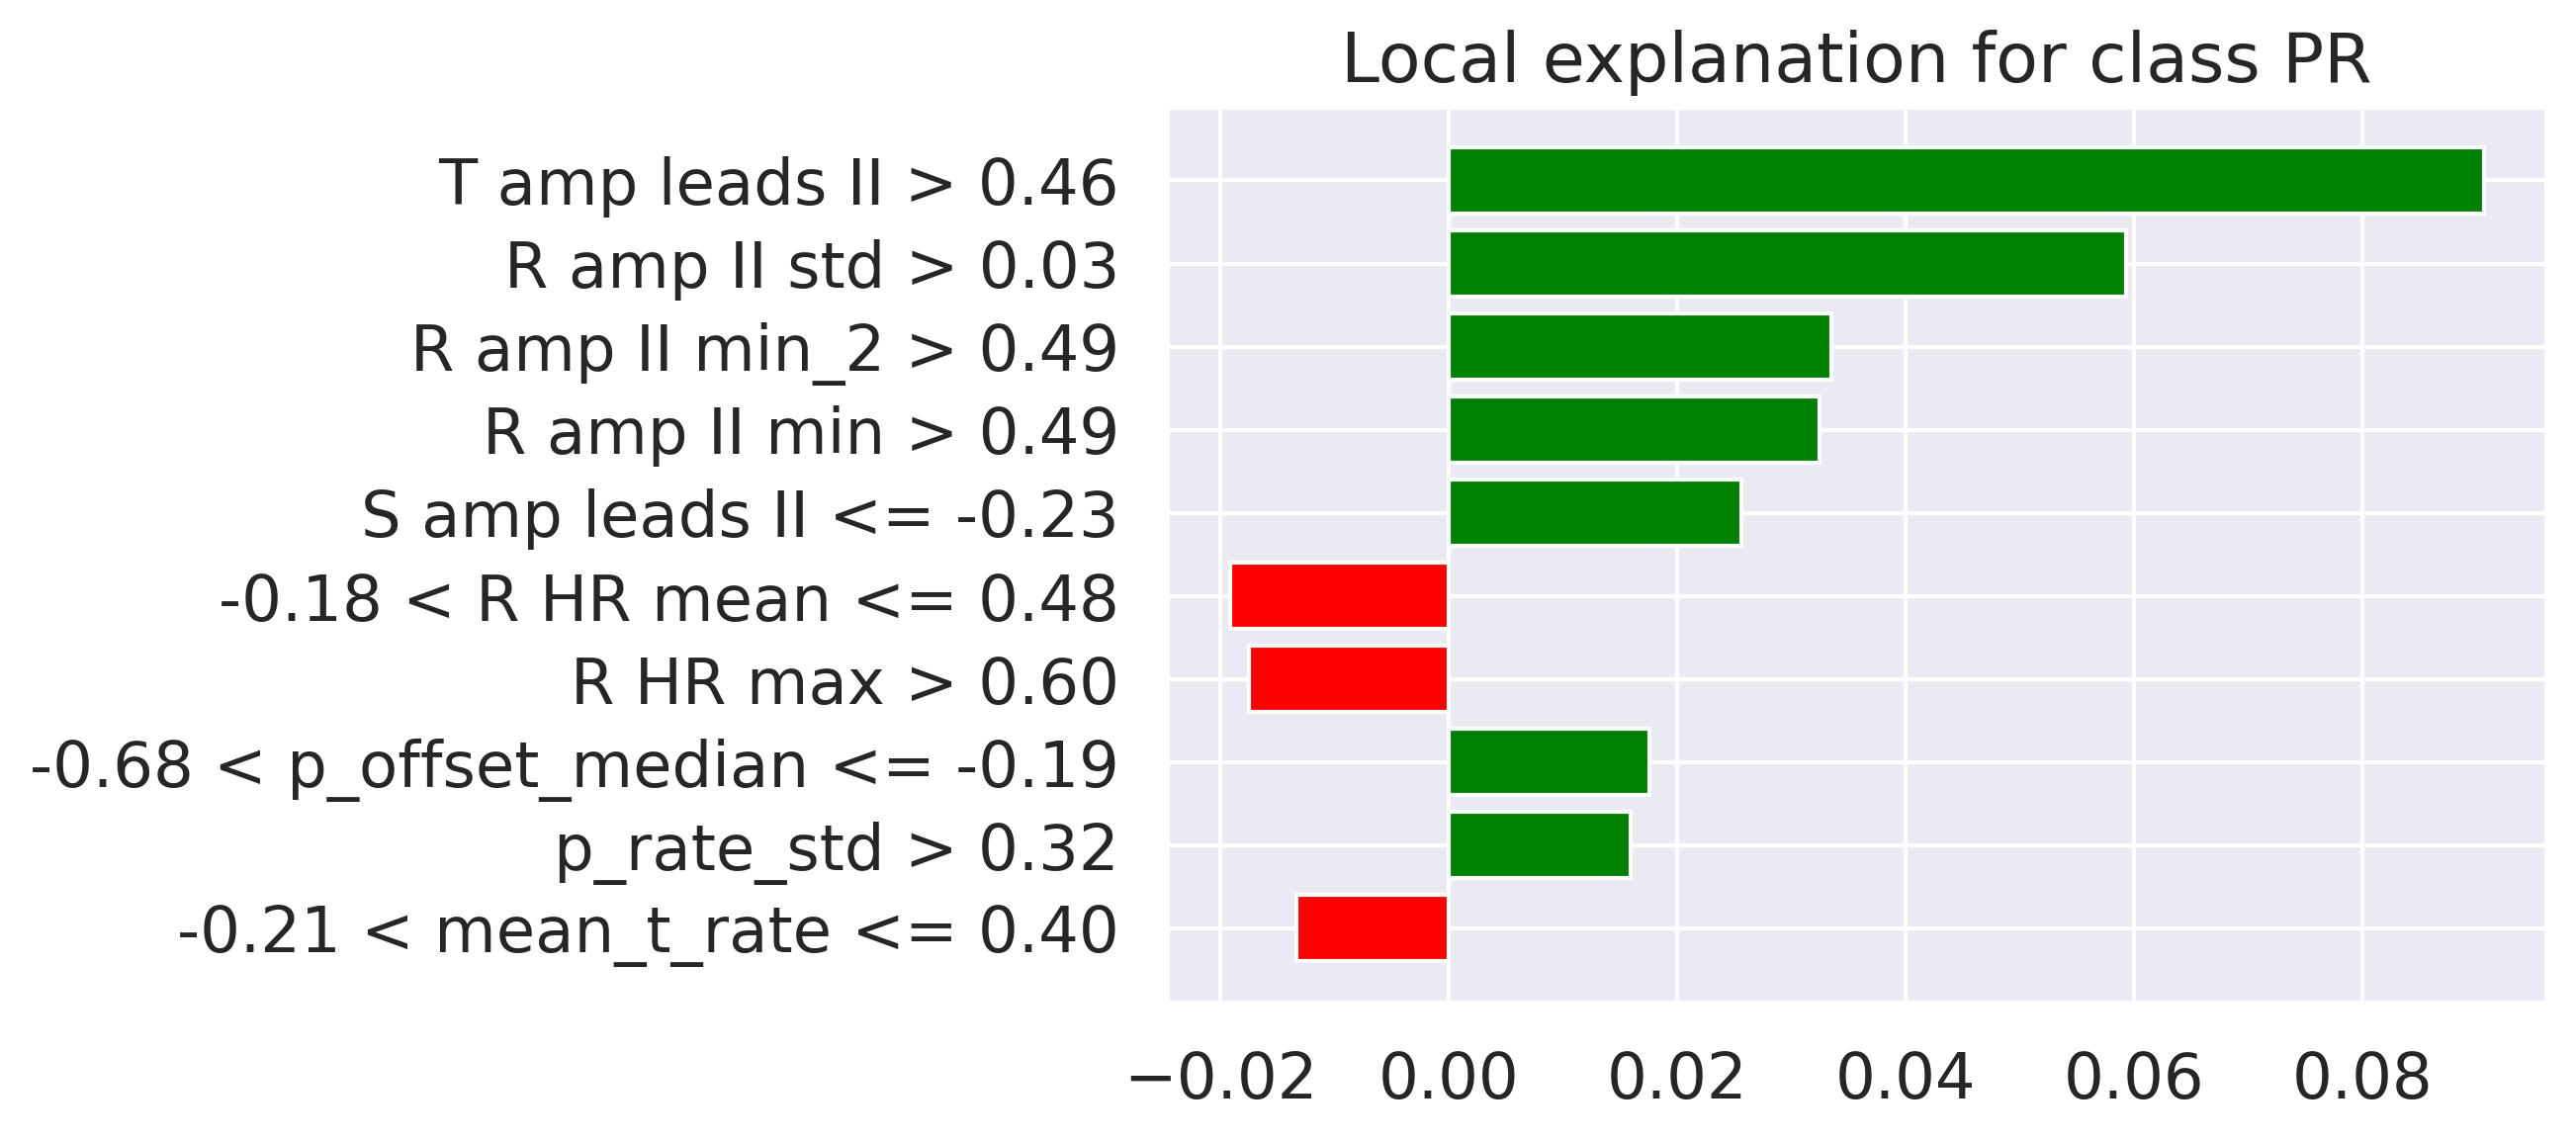
\includegraphics[width=1\textwidth]{Figures/pacing_rytm_2lead.png}
%    \caption{}
%    \label{fig:parameterregel}
%\end{figure}
%\begin{figure}[!bp]
%    \centering
%    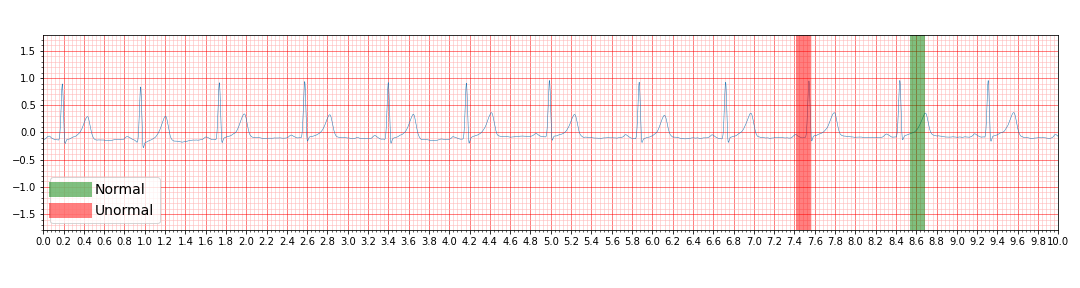
\includegraphics[width=1\textwidth]{Figures/Normal-V6.png}
%    \caption{The figure shows the explainability results from the Encoder 1D convolutional model. Sub-figure shows a 10 second ECG sequence of a normal ECG extracted from lead $II$ and sub-figure b show The vertical, transparent red bars in the plots indicate sections of the ECG that}
%    \label{fig:parameterregel}
%\end{figure}

The recurrent explainer, used on the Encoder model, was trained on $5000$ ECGs from the training data and then tested on an ECG from the test data. The ECG from the test data were abnormal and predicted correctly by the CNN model. The explanation model returned the channel/lead and the index of the sample/feature that was most important for the prediction by the Encoder. Figure \ref{fig:expl_cnn} shows the three most important features in lead aVR for the given test data.

\begin{figure}[!htp]
    \centering
    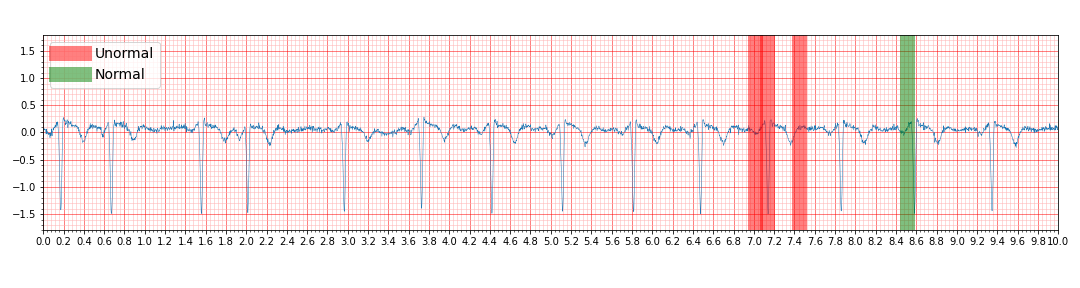
\includegraphics[width=1\textwidth]{Figures/Abnormal-aVR.png}
    \caption{The figure shows a 10 seconds long ECG-recording represented by the aVR-lead. The ECG is correctly classified as abnormal by a 1D CNN Encoder. The horizontal, transparent green and red lines mark the features in the ECG that are seen as normal and abnormal by LIMEs recurrent explanation model. The green line indicates the part of the ECG that contributes towards a normal classification while the red lines indicates the parts of the ECG that contributes towards an abnormal classification.}
    \label{fig:expl_cnn}
\end{figure}

\newpage

